%\addbibresource{/home/jorgsk/Dropbox/phdproject/bibtex/jorgsk.bib}
\subsection{Model of initial transcription}
Our goal was to obtain kinetic information of initial transcription. To this
end, it is necessary that the computational model is highly descriptive of the
process. The kinetic scheme of initial transcription considered here is given
in Figure \ref{fig:model}. For this model, we estimate the steps of NAC,
promoter escape, and unscrunching with commensurate abortive RNA release.

The dynamics of initial transcription is determined by the propensity
of RNAP to backtrack before reaching promoter escape
\cite{revyakin_abortive_2006}. If each backtracking event leads to the
abortive release of an RNA, the abortive probability (AP)
\cite{hsu_quantitative_1996} indicates the propensity for RNAP to backtrack.
Therefore, we constructed our kinetic model in such a way that the rate of
backtracking would reflect the abortive probability. By defining the rate
constant of backtracking in the model as 
\begin{equation*}
    b = \frac{NAC\cdot AP}{1-AP},
\end{equation*}
we specify that RNAP will backtrack with a rate that corresponds to a
probability of AP, and will proceed through NAC with a rate that corresponds
to 1-AP. With this definition of backtracking, it is given that the abortive
profile of the simulation will match the abortive profile obtained
experimentally. 

The abortive probabilities for a given ITS are obtained from Hsu et. al
\cite{hsu_initial_2006}. The rate of FL product synthesis upon promoter escape
is given by $e = NAC/d$ where d is the length of DNA from promoter escape
until runoff. Figure \ref{fig:parameter_estimation}A shows the initial
transcription kinetic scheme together with placeholder values for the the
estimated rates. Figure \ref{fig:parameter_estimation}B shows values obtained
for the N25 promoter when using $NAC=10/s$. 

To solve the kinetic scheme we use the direct method of the stochastic
simmulation algorithm \cite{gillespie_exact_1977} as implemented in the StocPY
software \cite{maarleveld_stochpy:_2013}. By using stochastic simulations, we
are able to simulate transcription to the level of single RNA polymerases,
which is required for fitting data to single-molecule experiments.

\begin{figure}
	\begin{center}
        \includegraphics{../illustrations/model.pdf}
	\end{center}
    \caption{Kinetic model scheme. From the open complex (OC)
    transcroption proceeds in cycles of nucleotide additions from one initial
    transcribing complex (IC) to the next, where each IC is identified by the
    length of the nascent RNA. For ICs with an 2nt RNA or more, there is a
    competition between the nucleotide addition cycle (NAC) and backtracking.
    Backtracking leads to a backtracked state from which unscrunching and
    abortive RNA release occurs.}
    \label{fig:model}
\end{figure}

\begin{figure}
	\begin{center}
        \includegraphics{../illustrations/parameter_estimation.pdf}
	\end{center}
    \caption{Estimated rates. NAC ($x$), promoter escape ($y$), and
    unscrunching and abortive release ($z$), and the backtracking rates
    $b_i(x)$ are estimated}
    \label{fig:parameter_estimation}
\end{figure}
%\bibliography{/home/jorgsk/Dropbox/phdproject/bibtex/jorgsk}
